\documentclass[10pt,a4paper]{article}

\usepackage[utf8]{inputenc}
\usepackage[french]{babel}
%\usepackage{lmodern}%pour un meilleur rendu des polices
\usepackage{verbatim}%du texte non interprt
\usepackage{amsmath,amssymb}%maths
\usepackage{graphicx}%images
\usepackage{xspace}
\usepackage{color}%Couleurs
\usepackage{listings}
\usepackage[a4paper, top= 2.5 cm, bottom = 2.5 cm, left = 2 cm, right = 1.5 cm] {geometry}
\usepackage{listings}
\usepackage{bbold}
\lstset{
  morekeywords={abort,abs,accept,access,all,and,array,at,begin,body,
      case,constant,declare,delay,delta,digits,do,else,elsif,end,entry,
      exception,exit,for,function,generic,goto,if,in,is,limited,loop,
      mod,new,not,null,of,or,others,out,package,pragma,private,
      procedure,raise,range,record,rem,renames,return,reverse,select,
      separate,subtype,task,terminate,then,type,use,when,while,with,
      xor,abstract,aliased,protected,requeue,tagged,until},
  sensitive=f,
  morecomment=[l]--,
  morestring=[d]",
  showstringspaces=false,
  basicstyle=\small\ttfamily,
  keywordstyle=\bf\small,
  commentstyle=\itshape,
  stringstyle=\sf,
  extendedchars=true,
  columns=[c]fixed, 
  language = C
}

%\usepackage{lastpage}%nombre de pages
%En tte et pied de page
\usepackage{fancyhdr}
\pagestyle{fancy}
\lhead{\sectionmark} 
\chead{}
\rhead{}
\lfoot{ENSIMAG 3A}
\cfoot{\textbf{Pilotage Bancaire}}
\rfoot{\thepage\ }
\renewcommand{\headrulewidth}{0pt}  
\renewcommand{\footrulewidth}{0.4pt}
%Page de garde
\makeatletter
\def\thickhrulefill{\leavevmode \leaders \hrule height 1pt\hfill \kern \z@}
\def\maketitle{%
  \thispagestyle{empty}%
  \begin{center}
  \begin{flushleft}
  \normalfont\LARGE \par
	  \end{flushleft}
	\vskip 5cm
	  \leavevmode
	  \normalfont
	  \thickhrulefill\par
	  \vskip 0.2cm
	  {\huge\@title\par}%
	  \vskip 0.1cm
  \thickhrulefill\par
	  \vskip 1cm
	  {\Large \@date\par}%
  \vskip 12cm
  {\Large \@author\par}%
  \end{center}%
	  \clearpage
}



\title{Pilotage Bancaire\\
{\em Crédit indexé sur le prix de l'énergie}}
\author{Edouard Baché - Guillaume Fuchs \\
Samy Mehenni - Guillaume Pelletier }
\date{Année 2013/2014}


\begin{document}
\maketitle
\newpage
\tableofcontents
\newpage

\section{Introduction}
La question écologique est aujourd'hui d'une importance cruciale. De nombreuses solutions sont mises en œuvres pour tenter de répondre à cette question qui concerne la planète entière.
D'autre part, depuis la crise de 2008, la finance éthique a connu une croissance phénoménale, et certaines banques, tel la Banque Populaire des Alpes (BPA), développent des produits en accord avec ce modèle.
C'est dans cette optique que notre équipe, a imaginé un crédit étant orienté vers le financement éthique et vers les investissement pour favoriser le développement durable. \\
Nous détaillerons dans les parties suivantes, le fonctionnement de ce crédit, ainsi que ses apports d'un point de vue éthique et enfin, nous fournirons une simulation complète de notre produit. Cependant, commençons par évaluer les enjeux d'un tel projet.

\section{Quels Enjeux ?}
Premièrement, comme pour tout crédit, il faut que le taux associé soit avantageux pour l'emprunteur, afin de pouvoir vendre ce prêt. D'autre part, il est nécessaire que notre produit financier génère des bénéfices assez important pour la banque. Notre équipe doit concevoir un produit étant capable de trouver un compromis afin de satisfaire les deux parties. Nous venons ainsi découvrir les \textbf{enjeux financiers} de notre produit, mais le crédit imaginé étant orienté vers le financement éthique, il devra répondre à certains critères. \\
En effet, ce prêt doit : 
\begin{itemize}
\item[•] Participer au développement durable. Notamment, ce genre de crédit ne sera accordé qu'aux clients ayant besoin de fonds pour réaliser des travaux liés aux améliorations écologiques (isolation,...). Les considérations écologiques liées au crédit sont à prendre très au sérieux.
\item[•] Prendre part au développement de la région. Que cela soit par l'amélioration du parc immobilier ou bien par la création d'emplois, la région est une partie intégrante du crédit.
\item[•] Assurer la transparence des investissements.
\end{itemize}



\section{Fonctionnement du crédit}
Ce chapitre s'intéressera à la définition du produit, d'un point de vue fonctionnel. Tout d'abord, nous introduirons le principe de ce prêt, ainsi que sa couverture. Dans un second temps, nous étudierons les autres composantes de sa tarification, pour fournir une évaluation complète.
\subsection{Principes du crédit}
L'idée de ce prêt est assez simpliste. Partons du postulat qu'un client particulier de la BPA, souhaite isoler son domicile afin de baisser fortement sa consommation de fioul. Il veut donc emprunter un certain montant pour financer ses travaux. De même, nous supposons qu'à chauffage constant de 19 degrés, l'emprunteur économiserait \textit{L} litres de fioul par mois. \\ Ainsi, la question qui se pose ici est : comment inclure les économies de l'investisseur dans les mensualités du prêt? \\
Nous avons alors pensé, que la meilleure manière de faire, serait simplement de considérer que chaque mensualité correspondrait au \underline{prix des économies réalisées}. \\
Nous proposons donc un \textbf{crédit à taux variable} indexé sur le \textbf{prix du fioul}. \\
Nous présentons ci-dessous un diagramme, représentant les flux générés par le produit, qui aidera à la compréhension de ce crédit : 
\begin{figure}[h!]
\begin{center}
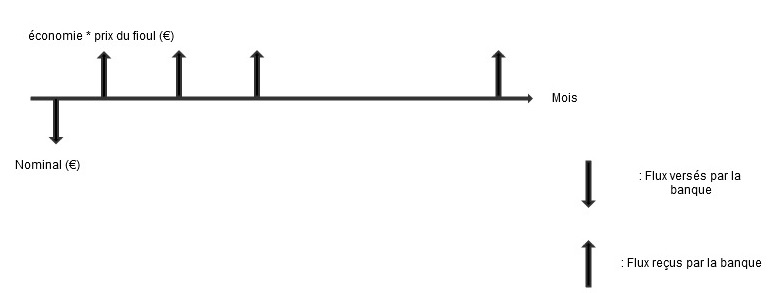
\includegraphics[scale=0.5]{flux.jpg}
\caption{Flux générés par le crédit}
\end{center}
\end{figure}
\vspace{2mm}
L'intérêt de crédit est double : 
\begin{itemize}
\item[•] Le client paye simplement ses économies de fioul, comme s'il payait sa facture mensuelle, ce qui lui donne l'impression de ne pas avoir de nouvelles charges à payer.
\item[•] L'utilisation d'une matière première, dans ce cas le fioul, permet à la banque d'assurer le côté éthique de son prêt (nous détaillerons ce point plus en détail dans une prochaine section).
\end{itemize}
\vspace{5mm}


Après avoir définit ce crédit, il convient d'étudier les risques qu'il induit, et surtout, d'étudier la couverture sur ce crédit spécifique.

\subsection{Risques induits par le sous-jacent et couverture}
Tout d'abord, il est clair que la volatilité du sous-jacent du crédit, le fioul, fait croître le \textbf{risque de défaut} de l'emprunteur\\
En effet, si le cours du fioul augmente fortement pendant la vie du crédit, il est probable que  l'investisseur se retrouve face à des mensualités qu'il est incapable de rembourser. Il est donc primordial de se couvrir contre ce genre de cas de figure. Ainsi, notre crédit sera muni d'un \textbf{cap à la hausse}, représentant le montant maximal à rembourser mensuellement par un client. Grâce à cette borne, nous immunisons l'emprunteur contre une hausse importante du prix du fioul, et la banque contre ce surplus de risque de défaut. 

\vspace{2mm} 
\textbf{Remarque : }Ce montant sera paramétrable par un agent de la banque. \\

Réciproquement, si le prix du fioul connaît une baisse importante, les mensualités seraient alors trop faibles et le remboursement du crédit serait d'autant plus long, ce qui est problématique pour l'institution financière accordant le prêt, et pour l'emprunteur. En effet, les mensualités étant plus faible, l'échéance du prêt s'allonge, ce qui est très gênant pour les deux parties. Donc, de manière identique au paragraphe précédent, nous munissons notre produit financier d'un \textbf{cap à la baisse}, représentant le montant minimal à rembourser mensuellement par l'emprunteur. Le calcul précis de cette borne sera détaillé plus loin dans notre document. \\

\subsection{Résumé sur le fonctionnement}
Résumons à présent les différents points définissants notre produit financer :
\begin{itemize}
\item[•] Notre produit est un crédit à taux variable, ce même taux dépendant du prix du fioul.
\item[•] Dans le cas où un client demande un prêt pour financer une économie d'énergie, les mensualités qu'il aura à rembourser correspondront aux prix des économies d'énergies mensuelles.
\item[•] Pour réduire l'impact lié à des variations trop importantes du prix du fioul, le produit sera "capé" à la hausse et à la baisse. Cela implique que les remboursements mensuels seront bornés entre deux valeurs.
\end{itemize}
\vspace{3mm}
Le diagramme ci dessous résume le fonctionnement de ce crédit :
\vspace{10mm}
\begin{figure}[h!]
\begin{center}
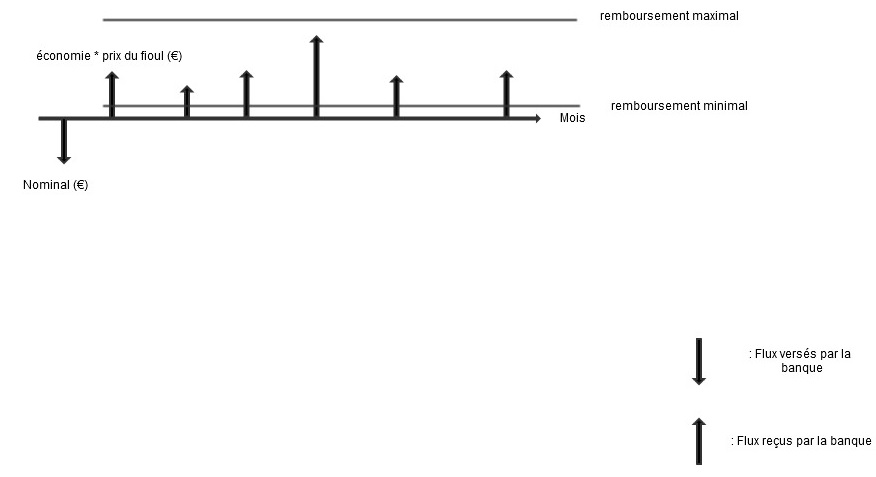
\includegraphics[scale=0.5]{resume_credit.jpg}
\caption{Fonctionnement général du produit}
\end{center}
\end{figure}
\vspace{3mm}
Nous venons ici de décrire le fonctionnement globale du produit que nous avons imaginé. Il est temps à présent d'essayer de tarifer ce crédit.

\subsection{Tarification du prêt}

\subsubsection{Taux de refinancement}

\subsubsection{Coûts de gestion}
% marginaux et complet (regréssion linéaire).
\subsubsection{Evaluation des pertes}

\subsubsection{Rendement des fonds propres}

\subsection{Clientèle visée}


\end{document}

